% SURGE-D architecture (Figure in Chapter 4). Build: pdflatex architecture.tex, then copy architecture.pdf to figures/.
% Shapes follow surge/model.py and surge/backbones.py (ViT-L numbers first, ViT-g second where they differ).
\documentclass[tikz,border=3pt]{standalone}
\usepackage[T1]{fontenc}
\usepackage{lmodern}   % Latin Modern, as in the thesis text
\usetikzlibrary{arrows.meta,calc}
\begin{document}
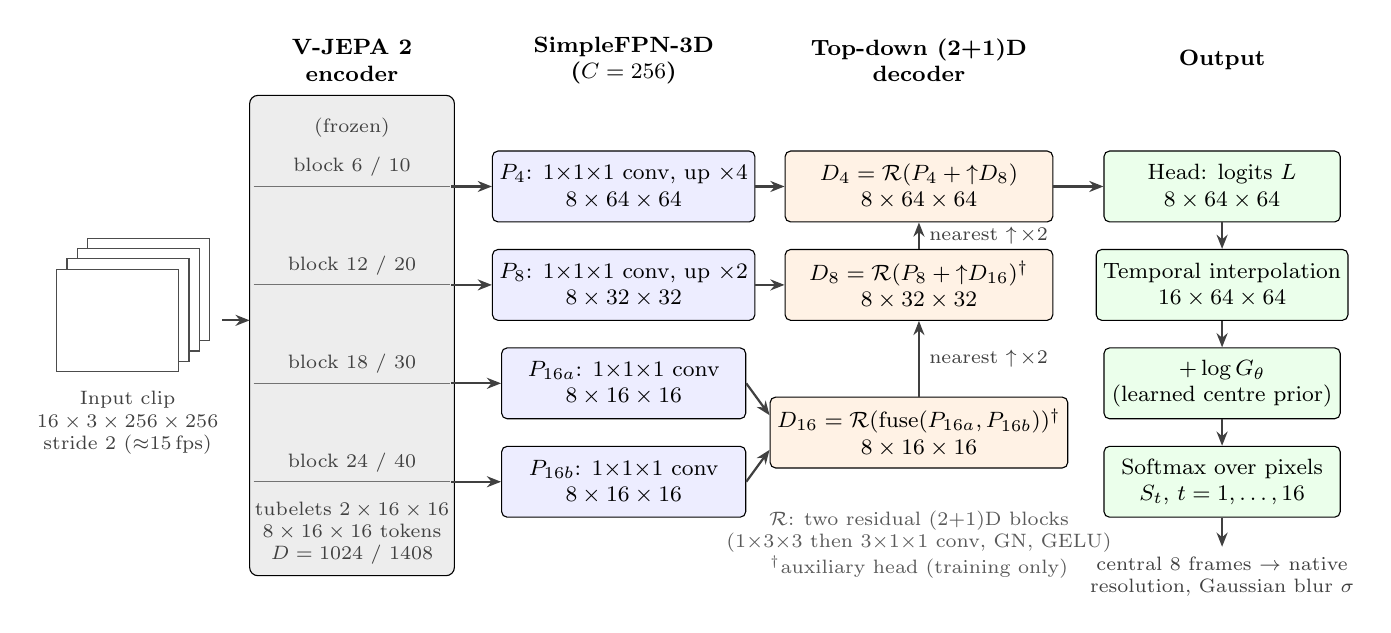
\begin{tikzpicture}[
  font=\footnotesize,
  >={Stealth[length=1.8mm,width=1.4mm]},
  box/.style={draw, rounded corners=2pt, align=center, inner sep=2.5pt, minimum height=9mm},
  fpn/.style={box, fill=blue!7, minimum width=31mm},
  dec/.style={box, fill=orange!10, minimum width=34mm},
  outb/.style={box, fill=green!8, minimum width=30mm},
  lab/.style={font=\scriptsize, text=black!75, align=center},
  grp/.style={font=\footnotesize\bfseries, align=center},
  arr/.style={->, thick, black!75},
]
\def\rA{4.6}\def\rB{3.35}\def\rC{2.1}\def\rD{0.85}
% ------------------------------------------------------------------ input clip
\foreach \i in {3,2,1,0} {
  \draw[fill=white, draw=black!70] ($(0.05,2.25)+(\i*0.13,\i*0.13)$) rectangle ++(1.55,1.3);
}
\node[lab] at (0.95,1.6) {Input clip\\$16\times3\times256\times256$\\stride 2 ($\approx$15\,fps)};
% ------------------------------------------------------------------ encoder
\node[draw, rounded corners=3pt, fill=black!7, minimum width=26mm, minimum height=61mm, anchor=south] at (3.8,-0.35) {};
\node[grp] at (3.8,6.2) {V-JEPA 2\\encoder};
\node[lab] at (3.8,5.35) {(frozen)};
\node[lab] at (3.8,0.2) {tubelets $2\times16\times16$\\$8\times16\times16$ tokens\\$D=1024$ / $1408$};
\foreach \y/\t in {\rA/{block 6 / 10}, \rB/{block 12 / 20}, \rC/{block 18 / 30}, \rD/{block 24 / 40}} {
  \draw[black!55] (2.55,\y) -- (5.05,\y);
  \node[lab, anchor=south] at (3.8,\y) {\t};
}
\draw[arr] (2.15,2.9) -- (2.5,2.9);
% ------------------------------------------------------------------ SimpleFPN-3D
\node[grp] at (7.25,6.2) {SimpleFPN-3D\\($C=256$)};
\node[fpn] (p4)   at (7.25,\rA) {$P_4$: $1{\times}1{\times}1$ conv, up $\times4$\\$8\times64\times64$};
\node[fpn] (p8)   at (7.25,\rB) {$P_8$: $1{\times}1{\times}1$ conv, up $\times2$\\$8\times32\times32$};
\node[fpn] (p16a) at (7.25,\rC) {$P_{16a}$: $1{\times}1{\times}1$ conv\\$8\times16\times16$};
\node[fpn] (p16b) at (7.25,\rD) {$P_{16b}$: $1{\times}1{\times}1$ conv\\$8\times16\times16$};
\foreach \n/\y in {p4/\rA, p8/\rB, p16a/\rC, p16b/\rD} { \draw[arr] (5.06,\y) -- (\n.west); }
% ------------------------------------------------------------------ decoder
\node[grp] at (11.0,6.2) {Top-down (2+1)D\\decoder};
\node[dec] (d4)  at (11.0,\rA) {$D_4=\mathcal{R}(P_4+{\uparrow}D_8)$\\$8\times64\times64$};
\node[dec] (d8)  at (11.0,\rB) {$D_8=\mathcal{R}(P_8+{\uparrow}D_{16})^{\dagger}$\\$8\times32\times32$};
\node[dec] (d16) at (11.0,1.475) {$D_{16}=\mathcal{R}(\mathrm{fuse}(P_{16a},P_{16b}))^{\dagger}$\\$8\times16\times16$};
\draw[arr] (p4.east) -- (d4.west);
\draw[arr] (p8.east) -- (d8.west);
\draw[arr] (p16a.east) -- ($(d16.west)+(0,0.22)$);
\draw[arr] (p16b.east) -- ($(d16.west)+(0,-0.22)$);
\draw[arr] (d16.north) -- node[lab, right] {nearest $\uparrow\!\times2$} (d8.south);
\draw[arr] (d8.north) -- node[lab, right] {nearest $\uparrow\!\times2$} (d4.south);
\node[lab, text=black!65] at (11.0,0.05) {$\mathcal{R}$: two residual (2+1)D blocks\\($1{\times}3{\times}3$ then $3{\times}1{\times}1$ conv, GN, GELU)\\$^{\dagger}$auxiliary head (training only)};
% ------------------------------------------------------------------ output
\node[grp] at (14.85,6.2) {Output};
\node[outb] (head)  at (14.85,\rA) {Head: logits $L$\\$8\times64\times64$};
\node[outb] (tint)  at (14.85,\rB) {Temporal interpolation\\$16\times64\times64$};
\node[outb] (prior) at (14.85,\rC) {$+\log G_\theta$\\(learned centre prior)};
\node[outb] (soft)  at (14.85,\rD) {Softmax over pixels\\$S_t$, $t=1,\dots,16$};
\node[lab] (post) at (14.85,-0.35) {central 8 frames $\to$ native\\resolution, Gaussian blur $\sigma$};
\draw[arr] (d4.east) -- (head.west);
\draw[arr] (head.south) -- (tint.north);
\draw[arr] (tint.south) -- (prior.north);
\draw[arr] (prior.south) -- (soft.north);
\draw[arr] (soft.south) -- (post.north);
\end{tikzpicture}
\end{document}
